\section{Results}\label{sec:results}

\subsection{Boundary Accuracy}\label{sec:res-f1}
Table~\ref{tab:f1} and Figure~\ref{fig:f1} give boundary F1 against the MorphScore gold boundaries for every method and language; the precision and recall behind them are in Tables~\ref{tab:precision} and~\ref{tab:recall} of the appendix, and Figure~\ref{fig:pr} places every method in the precision--recall plane.

\begin{table}[!ht]
\centering
\caption{Boundary F1 (\%) against the lemma-derived morpheme boundaries of MorphScore, all unique word forms. Mean $\pm$ standard deviation over three training seeds; best per language in bold.}
\label{tab:f1}
\small
\setlength{\tabcolsep}{4pt}
\begin{tabular}{lccccc}
\toprule
System & English & Spanish & Danish & Tamil & Turkish \\
\midrule
BPE, free marker & 40.0\,{\scriptsize$\pm$1.6} & 18.7\,{\scriptsize$\pm$0.8} & 24.3\,{\scriptsize$\pm$0.8} & 4.4\,{\scriptsize$\pm$2.3} & 35.0\,{\scriptsize$\pm$1.9} \\
POS-weighted BPE & 43.4\,{\scriptsize$\pm$1.6} & 18.9\,{\scriptsize$\pm$0.8} & 24.5\,{\scriptsize$\pm$0.5} & 6.2\,{\scriptsize$\pm$2.3} & 35.0\,{\scriptsize$\pm$1.6} \\
\quad transitions only & 43.4\,{\scriptsize$\pm$1.6} & 18.9\,{\scriptsize$\pm$0.8} & 24.5\,{\scriptsize$\pm$0.5} & 6.2\,{\scriptsize$\pm$2.3} & 35.1\,{\scriptsize$\pm$1.6} \\
\quad penalty only & 42.0\,{\scriptsize$\pm$1.3} & 18.7\,{\scriptsize$\pm$0.8} & 24.4\,{\scriptsize$\pm$1.0} & 4.4\,{\scriptsize$\pm$2.3} & 34.9\,{\scriptsize$\pm$1.9} \\
\addlinespace[2pt]
Content-word-weighted BPE & 43.9\,{\scriptsize$\pm$0.2} & 16.5\,{\scriptsize$\pm$0.3} & 27.8\,{\scriptsize$\pm$0.7} & 22.2\,{\scriptsize$\pm$1.1} & 34.2\,{\scriptsize$\pm$0.4} \\
Lemma2Word + BPE & \textbf{59.9\,{\scriptsize$\pm$0.1}} & \textbf{36.3\,{\scriptsize$\pm$0.1}} & \textbf{43.8\,{\scriptsize$\pm$0.3}} & \textbf{52.9\,{\scriptsize$\pm$0.4}} & \textbf{48.7\,{\scriptsize$\pm$0.1}} \\
BPE, word-initial marker & 25.5\,{\scriptsize$\pm$0.4} & 6.7\,{\scriptsize$\pm$0.5} & 13.1\,{\scriptsize$\pm$0.1} & 7.5\,{\scriptsize$\pm$0.3} & 40.8\,{\scriptsize$\pm$0.4} \\
Unigram LM & 54.3\,{\scriptsize$\pm$0.5} & 29.0\,{\scriptsize$\pm$0.0} & 35.1\,{\scriptsize$\pm$0.5} & 43.0\,{\scriptsize$\pm$0.8} & 46.5\,{\scriptsize$\pm$0.4} \\
\bottomrule
\end{tabular}
\end{table}


\begin{figure}[!ht]
\centering
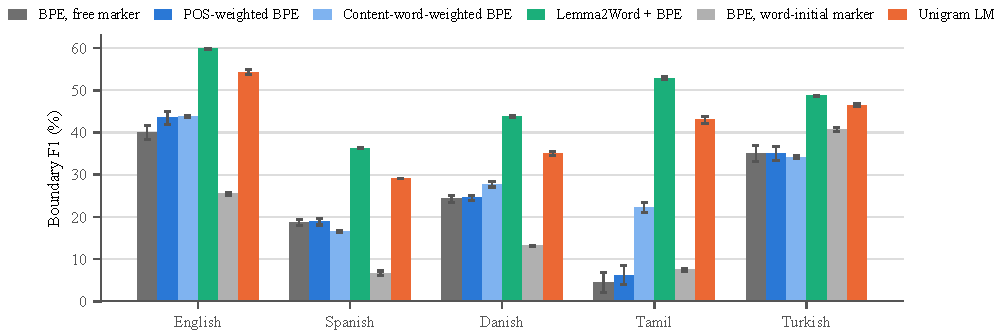
\includegraphics[width=\linewidth]{figures/fig_f1.pdf}
\caption{Boundary F1 (\%) of the six main tokenizers in five languages. Bars are means over three training seeds and error bars span one standard deviation.}
\label{fig:f1}
\end{figure}

Lemma2Word has the highest F1 in every language, from \nFLtwSpanish\% in Spanish to \nFLtwEnglish\% in English.
The unigram model is second everywhere, and ahead of every BPE variant by a wide margin in Tamil (\nFUniTamil\% against \nFBpeTamil\% for free-marker BPE).
The POS-weighted BPE differs from its unweighted base by about three points in English (\nFPosEnglish\% against \nFBpeEnglish\%) and by less than one point in Spanish, Danish and Turkish; only the English difference exceeds the seed-to-seed standard deviation.
Its two ablations show that the transition term carries the whole effect, since \emph{transitions only} reproduces the full variant to the first decimal and \emph{penalty only} is indistinguishable from the unweighted base.
The content-word weighting raises F1 from \nFBpeTamil\% to \nFPosContentTamil\% in Tamil and by about three points in English and Danish, and lowers it in Spanish and Turkish.
The BPE with a word-initial marker, the convention of SentencePiece, has the lowest F1 in four languages; with the whole word and its marker available as a single token, it places fewer boundaries inside words than the free-marker variant (recall \nRHfBpeSpanish\% against \nRBpeSpanish\% in Spanish).

\begin{figure}[!ht]
\centering
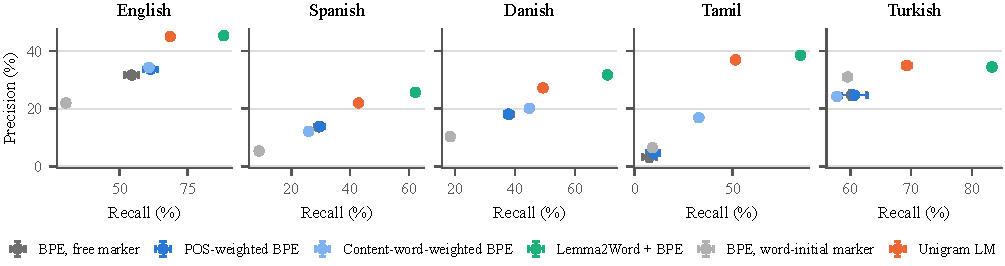
\includegraphics[width=\linewidth]{figures/fig_pr.pdf}
\caption{Boundary precision against recall per language. Points are means over three seeds and error bars span one standard deviation; most are smaller than the markers.}
\label{fig:pr}
\end{figure}

\subsection{What the Part-of-Speech Weighting Changes}\label{sec:res-pos}
The weighting of Section~\ref{sec:posbpe} only changes the score of merges that attach a word to the space after it.
Table~\ref{tab:span} shows what those merges produce on held-out text.
Between \nSpanShareBpeTurkish\% (Turkish) and \nSpanShareBpeSpanish\% (Spanish) of word boundaries end up inside a token under plain free-marker BPE, and the POS weighting leaves those shares almost unchanged except in Tamil, where it lowers the share from \nSpanShareBpeTamil\% to \nSpanSharePosTamil\%\footnote{Seed 0; the three-seed mean of the share of tokens that span a boundary falls from \nCrossBpeTamil\% to \nCrossPosTamil\% (Table~\ref{tab:cross}).}.
The transitions spanned are the ones BPE spans anyway: adposition followed by determiner in English (\texttt{of\textvisiblespace the\textvisiblespace}), determiner followed by noun in Spanish, noun followed by adposition in Danish.
The mean probability of the transition at a spanned boundary is within two points of the mean over all boundaries for every language and every variant, with or without the weighting.
Frequency decides which boundaries a token crosses, and the transition probabilities, which are themselves frequencies of tag pairs, add nothing that the symbol counts do not already contain.

\begin{table}[!ht]
\centering
\caption{Word boundaries spanned by a token on held-out text: share of boundaries (\%), mean probability (\%) of the POS transition at spanned boundaries, and the same mean over all boundaries. Seed 0; the most frequent spanned transition and token are shown for the POS-weighted model.}
\label{tab:span}
\footnotesize
\setlength{\tabcolsep}{3.5pt}
\begin{tabular}{llccclc}
\toprule
Language & System & spanned (\%) & $P$, spanned & $P$, all & top transition & top token \\
\midrule
English & BPE, free marker & 45.2 & 23.3 & 22.1 & ADP$\to$DET & \texttt{in\textvisiblespace{}the\textvisiblespace{}} \\
 & POS-weighted BPE & 42.6 & 23.5 & 22.1 & ADP$\to$DET & \texttt{of\textvisiblespace{}the\textvisiblespace{}} \\
 & Content-word-weighted BPE & 33.2 & 24.4 & 22.1 & ADP$\to$DET & \texttt{of\textvisiblespace{}the\textvisiblespace{}} \\
\addlinespace[2pt]
Spanish & BPE, free marker & 54.1 & 32.3 & 28.2 & DET$\to$NOUN & \texttt{a\textvisiblespace{}de\textvisiblespace{}} \\
 & POS-weighted BPE & 54.1 & 32.3 & 28.2 & DET$\to$NOUN & \texttt{a\textvisiblespace{}de\textvisiblespace{}} \\
 & Content-word-weighted BPE & 43.5 & 33.8 & 28.2 & DET$\to$NOUN & \texttt{en\textvisiblespace{}la\textvisiblespace{}} \\
\addlinespace[2pt]
Danish & BPE, free marker & 41.3 & 21.1 & 22.4 & NOUN$\to$ADP & \texttt{en\textvisiblespace{}i\textvisiblespace{}} \\
 & POS-weighted BPE & 41.4 & 21.1 & 22.4 & NOUN$\to$ADP & \texttt{en\textvisiblespace{}i\textvisiblespace{}} \\
 & Content-word-weighted BPE & 31.0 & 20.9 & 22.4 & NOUN$\to$ADP & \texttt{er\textvisiblespace{}i\textvisiblespace{}} \\
\addlinespace[2pt]
Tamil & BPE, free marker & 54.1 & 24.4 & 24.9 & NOUN$\to$NOUN & \tamil{ு}\textvisiblespace{}\tamil{ப} \\
 & POS-weighted BPE & 39.5 & 25.0 & 24.9 & NOUN$\to$NOUN & \tamil{ு}\textvisiblespace{}\tamil{ப} \\
 & Content-word-weighted BPE & 7.4 & 26.5 & 24.9 & NOUN$\to$NOUN & \tamil{ப்}\textvisiblespace{}\tamil{ப} \\
\addlinespace[2pt]
Turkish & BPE, free marker & 15.5 & 22.3 & 25.0 & NOUN$\to$CCONJ & \texttt{i\textvisiblespace{}ve\textvisiblespace{}} \\
 & POS-weighted BPE & 15.2 & 22.5 & 25.0 & NOUN$\to$CCONJ & \texttt{i\textvisiblespace{}ve\textvisiblespace{}} \\
 & Content-word-weighted BPE & 9.0 & 23.7 & 25.0 & NOUN$\to$CCONJ & \texttt{i\textvisiblespace{}ve\textvisiblespace{}} \\
\addlinespace[2pt]
\bottomrule
\end{tabular}
\end{table}


\subsection{Content-Word Weighting}\label{sec:res-content}
Doubling the weight of merges inside nouns, proper nouns, verbs and adjectives has the effect it was designed to have, a vocabulary that spends more of its budget on whole content words, and that effect helps or hurts depending on the language.
It lowers the share of tokens that span a word boundary everywhere (Table~\ref{tab:cross}) and raises recall in Tamil from \nRBpeTamil\% to \nRPosContentTamil\%, where plain BPE almost never cuts at the stem boundary.
In Spanish and Turkish it lowers recall, because the whole-word tokens it buys replace the suffix tokens that plain BPE learns there.
The weight of 2 was fixed in advance; a sweep over it would turn the variant into a tuned method and was not run.

\subsection{Lemma2Word}\label{sec:res-l2w}
Table~\ref{tab:l2w} separates the lexicon variant, which uses nothing beyond what it learned from the training text, from the online variant, which lemmatizes every evaluation word with Stanza, and reports both on all forms, on forms absent from the training text, and on forms from the Universal Dependencies test split.

\begin{table}[!ht]
\centering
\caption{Lemma2Word boundary recall and precision (\%) by word subset: all unique forms, forms absent from the tokenizer's training text, and forms from the UD test split. \emph{Lexicon} uses only boundaries and affixes learned from the training text; \emph{online} also lemmatizes the evaluation word with Stanza at tokenization time. Mean over three seeds.}
\label{tab:l2w}
\small
\setlength{\tabcolsep}{3.5pt}
\begin{tabular}{llcccccc}
\toprule
 & & \multicolumn{2}{c}{all} & \multicolumn{2}{c}{unseen} & \multicolumn{2}{c}{UD test} \\
\cmidrule(lr){3-4}\cmidrule(lr){5-6}\cmidrule(lr){7-8}
Language & Variant & R & P & R & P & R & P \\
\midrule
English & lexicon & 88.2 & 45.3 & 73.7 & 30.3 & 84.0 & 37.2 \\
 & online & 98.2 & 50.9 & 98.2 & 41.1 & 91.1 & 40.9 \\
 & BPE, free marker & 54.4 & 31.6 & 54.5 & 25.5 & 49.2 & 24.8 \\
\addlinespace[2pt]
Spanish & lexicon & 62.2 & 25.6 & 40.2 & 15.3 & 48.1 & 18.3 \\
 & online & 99.1 & 39.0 & 99.1 & 35.4 & 94.8 & 34.2 \\
 & BPE, free marker & 29.4 & 13.7 & 35.8 & 14.7 & 31.8 & 13.2 \\
\addlinespace[2pt]
Danish & lexicon & 70.8 & 31.7 & 49.5 & 17.9 & 65.5 & 27.2 \\
 & online & 97.2 & 43.6 & 97.1 & 35.3 & 88.0 & 37.0 \\
 & BPE, free marker & 37.9 & 17.9 & 41.0 & 15.9 & 38.0 & 16.7 \\
\addlinespace[2pt]
Tamil & lexicon & 84.5 & 38.5 & 74.2 & 27.4 & 80.6 & 34.7 \\
 & online & 97.6 & 46.3 & 97.7 & 38.5 & 91.5 & 39.9 \\
 & BPE, free marker & 7.4 & 3.2 & 7.0 & 2.5 & 5.9 & 2.4 \\
\addlinespace[2pt]
Turkish & lexicon & 83.3 & 34.4 & 81.7 & 31.2 & 82.7 & 32.0 \\
 & online & 88.6 & 37.6 & 88.4 & 34.8 & 89.1 & 35.6 \\
 & BPE, free marker & 60.2 & 24.7 & 60.5 & 23.2 & 60.4 & 23.2 \\
\addlinespace[2pt]
\bottomrule
\end{tabular}
\end{table}


On all forms, the lexicon variant raises recall over free-marker BPE from \nRBpeEnglish\% to \nLtwLexiconAllREnglish\% in English, from \nRBpeTamil\% to \nLtwLexiconAllRTamil\% in Tamil, and by 23 to 34 points in the other three languages, while precision rises as well, since the pieces it hands to BPE are shorter and BPE places fewer boundaries inside them.
On unseen forms, where only the affix inventories can act, recall is \nLtwLexiconUnseenREnglish\% in English and \nLtwLexiconUnseenRTamil\% in Tamil, and it shrinks to a few points in Spanish and Danish, whose inflectional suffixes are short and ambiguous with word-final letter sequences, so that the 20-occurrence threshold admits few of them.
The online variant recovers almost every gold boundary (\nLtwOnlineAllRSpanish\% recall in Spanish), which is expected, because the gold boundaries are themselves derived from lemmas and, on forms from the treebank training split, the lemmatizer can return the gold lemma from memory.
On the test-split forms, which the lemmatizer never saw, recall is lower but still between \nLtwOnlineTestRDanish\% and \nLtwOnlineTestRSpanish\%.
The precision of the online variant stays below 51\% because BPE goes on splitting inside the pieces; the gold standard records only the stem boundary.

\subsection{Compression and Stability}\label{sec:res-compression}
Table~\ref{tab:tpw} reports tokens per word on held-out text.
The POS weighting changes compression by less than one percent.
Lemma2Word needs \nTpwLtwEnglish{} tokens per word in English against \nTpwBpeEnglish{} for free-marker BPE (four percent more) and \nTpwLtwSpanish{} against \nTpwBpeSpanish{} in Spanish (eight percent more), and it is still more compact than the unigram model in every language but Tamil.
The two reference tokenizers, which never cross a word boundary, need more tokens per word than free-marker BPE in the three European languages and fewer in Tamil and Turkish, where free-marker BPE spends part of its budget on tokens that span frequent word pairs.

\begin{table}[!ht]
\centering
\caption{Tokens per whitespace word on held-out Wikipedia paragraphs (lower is more compact).}
\label{tab:tpw}
\small
\setlength{\tabcolsep}{4pt}
\begin{tabular}{lccccc}
\toprule
System & English & Spanish & Danish & Tamil & Turkish \\
\midrule
BPE, free marker & 1.481\,{\scriptsize$\pm$0.002} & 1.413\,{\scriptsize$\pm$0.002} & 1.606\,{\scriptsize$\pm$0.002} & 2.242\,{\scriptsize$\pm$0.005} & 1.962\,{\scriptsize$\pm$0.002} \\
POS-weighted BPE & 1.470\,{\scriptsize$\pm$0.001} & \textbf{1.412\,{\scriptsize$\pm$0.001}} & \textbf{1.604\,{\scriptsize$\pm$0.002}} & 2.215\,{\scriptsize$\pm$0.006} & 1.938\,{\scriptsize$\pm$0.025} \\
\quad transitions only & 1.470\,{\scriptsize$\pm$0.001} & 1.412\,{\scriptsize$\pm$0.001} & 1.604\,{\scriptsize$\pm$0.002} & 2.215\,{\scriptsize$\pm$0.006} & 1.938\,{\scriptsize$\pm$0.025} \\
\quad penalty only & \textbf{1.470\,{\scriptsize$\pm$0.001}} & 1.413\,{\scriptsize$\pm$0.002} & 1.605\,{\scriptsize$\pm$0.002} & 2.243\,{\scriptsize$\pm$0.005} & 1.962\,{\scriptsize$\pm$0.003} \\
\addlinespace[2pt]
Content-word-weighted BPE & 1.486\,{\scriptsize$\pm$0.002} & 1.423\,{\scriptsize$\pm$0.002} & 1.619\,{\scriptsize$\pm$0.001} & 2.150\,{\scriptsize$\pm$0.012} & 1.998\,{\scriptsize$\pm$0.003} \\
Lemma2Word + BPE & 1.538\,{\scriptsize$\pm$0.001} & 1.531\,{\scriptsize$\pm$0.002} & 1.703\,{\scriptsize$\pm$0.001} & 2.376\,{\scriptsize$\pm$0.002} & 2.080\,{\scriptsize$\pm$0.010} \\
BPE, word-initial marker & 1.555\,{\scriptsize$\pm$0.001} & 1.565\,{\scriptsize$\pm$0.000} & 1.713\,{\scriptsize$\pm$0.001} & \textbf{2.042\,{\scriptsize$\pm$0.001}} & \textbf{1.883\,{\scriptsize$\pm$0.002}} \\
Unigram LM & 1.609\,{\scriptsize$\pm$0.001} & 1.607\,{\scriptsize$\pm$0.002} & 1.778\,{\scriptsize$\pm$0.004} & 2.177\,{\scriptsize$\pm$0.006} & 2.004\,{\scriptsize$\pm$0.004} \\
\bottomrule
\end{tabular}
\end{table}


Stability across training samples (Tables~\ref{tab:jaccard} and~\ref{tab:agreement} in the appendix) separates the methods less than accuracy does.
Two vocabularies learned from different samples share between 62\% and 79\% of their entries by the Jaccard measure, and two tokenizers of the same method segment the same held-out text with a boundary agreement of 88\% to 97\%.
The POS weighting does not improve either number; in Turkish it lowers vocabulary overlap from \nJacBpeTurkish\% to \nJacPosTurkish\% with a standard deviation of \nJacPosTurkishSd{} points, the least stable entry in the table.
The unigram model has the lowest vocabulary overlap in every language and an agreement comparable to the others, so its vocabularies vary in the rare entries that seldom appear in held-out text.

\subsection{Vocabulary Budget}\label{sec:res-sweep}
Figure~\ref{fig:sweep} repeats the comparison at budgets of 2,000 and 32,000 types with seed 0.
The ordering of the methods is the same at every budget.
Lemma2Word gains with the budget in every language, from \nSweepFLtwEnglishVTwoK\% to \nSweepFLtwEnglishVThirtyTwoK\% in English, because a larger vocabulary leaves its pieces whole more often.
The unigram model loses accuracy at 32,000 types in English, Tamil and Turkish, where that budget exceeds the number of word types a 3,000-paragraph sample can support and whole words enter the vocabulary.
The gap between the POS-weighted and the unweighted BPE stays within three points at every budget.

\begin{figure}[!ht]
\centering
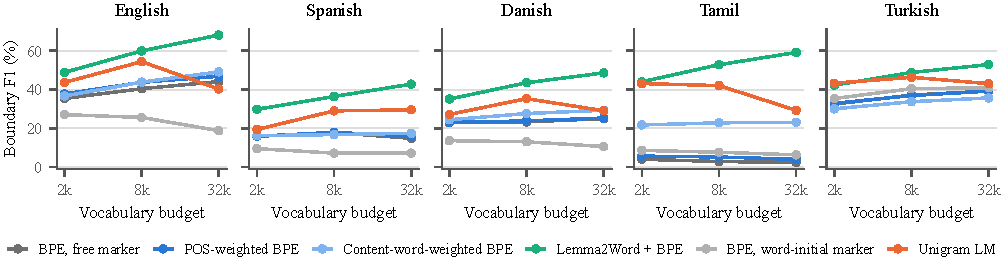
\includegraphics[width=\linewidth]{figures/fig_sweep.pdf}
\caption{Boundary F1 (\%) at vocabulary budgets of 2,000, 8,000 and 32,000 types, seed 0.}
\label{fig:sweep}
\end{figure}

\subsection{Language-Model Probe}\label{sec:res-lm}
Table~\ref{tab:bpc} and Figure~\ref{fig:bpc} report the bits per character of the language model trained on each tokenizer's output, with one model per tokenizer seed.
The seed-to-seed standard deviation is below 0.01 bits for most entries and 0.03 at worst, so differences of a few hundredths are reliable at this scale.

\begin{table}[!ht]
\centering
\caption{Bits per character of a 7M-parameter language model trained for six passes over the same text with each tokenizer (lower is better). Mean $\pm$ standard deviation over the three tokenizer seeds.}
\label{tab:bpc}
\small
\setlength{\tabcolsep}{4pt}
\begin{tabular}{lccccc}
\toprule
System & English & Spanish & Danish & Tamil & Turkish \\
\midrule
BPE, free marker & 2.807\,{\scriptsize$\pm$0.002} & 2.689\,{\scriptsize$\pm$0.003} & 2.878\,{\scriptsize$\pm$0.001} & 2.848\,{\scriptsize$\pm$0.006} & 2.963\,{\scriptsize$\pm$0.002} \\
POS-weighted BPE & 2.785\,{\scriptsize$\pm$0.001} & 2.687\,{\scriptsize$\pm$0.001} & 2.874\,{\scriptsize$\pm$0.001} & 2.819\,{\scriptsize$\pm$0.005} & 2.935\,{\scriptsize$\pm$0.032} \\
\quad transitions only & 2.785\,{\scriptsize$\pm$0.001} & 2.687\,{\scriptsize$\pm$0.001} & 2.874\,{\scriptsize$\pm$0.002} & 2.819\,{\scriptsize$\pm$0.005} & 2.935\,{\scriptsize$\pm$0.032} \\
\quad penalty only & 2.786\,{\scriptsize$\pm$0.002} & 2.689\,{\scriptsize$\pm$0.002} & 2.876\,{\scriptsize$\pm$0.001} & 2.849\,{\scriptsize$\pm$0.006} & 2.963\,{\scriptsize$\pm$0.003} \\
\addlinespace[2pt]
Content-word-weighted BPE & 2.794\,{\scriptsize$\pm$0.001} & 2.680\,{\scriptsize$\pm$0.003} & 2.868\,{\scriptsize$\pm$0.001} & 2.737\,{\scriptsize$\pm$0.015} & 2.995\,{\scriptsize$\pm$0.003} \\
Lemma2Word + BPE & 2.887\,{\scriptsize$\pm$0.003} & 2.861\,{\scriptsize$\pm$0.004} & 3.007\,{\scriptsize$\pm$0.001} & 2.983\,{\scriptsize$\pm$0.002} & 3.096\,{\scriptsize$\pm$0.011} \\
BPE, word-initial marker & 2.715\,{\scriptsize$\pm$0.003} & 2.674\,{\scriptsize$\pm$0.006} & 2.909\,{\scriptsize$\pm$0.003} & 2.611\,{\scriptsize$\pm$0.001} & 2.808\,{\scriptsize$\pm$0.004} \\
Unigram LM & \textbf{2.531\,{\scriptsize$\pm$0.006}} & \textbf{2.473\,{\scriptsize$\pm$0.011}} & \textbf{2.704\,{\scriptsize$\pm$0.007}} & \textbf{2.524\,{\scriptsize$\pm$0.003}} & \textbf{2.694\,{\scriptsize$\pm$0.003}} \\
\bottomrule
\end{tabular}
\end{table}


\begin{figure}[!ht]
\centering
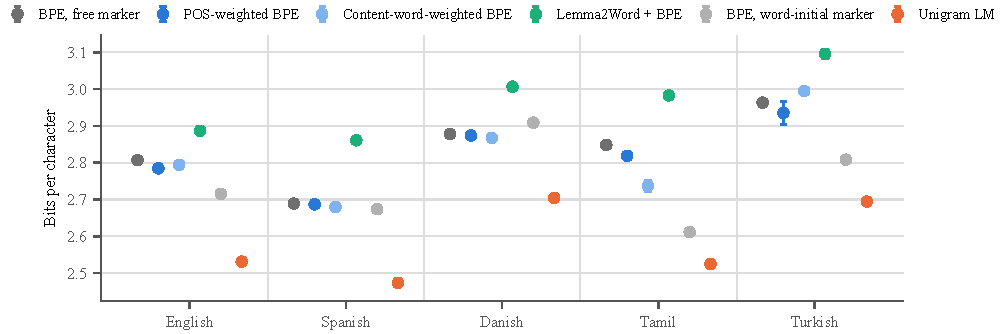
\includegraphics[width=\linewidth]{figures/fig_bpc.pdf}
\caption{Bits per character of a 7M-parameter language model trained for six passes over the same text with each tokenizer (lower is better). Points are means over the three tokenizer seeds and error bars span one standard deviation; the vertical axis starts at 2.4 bits so that the differences are visible.}
\label{fig:bpc}
\end{figure}

The ordering by bits per character is not the ordering by boundary F1.
The unigram model, second by F1, is first by a wide margin in every language, at \nBpcUniEnglish{} bits against \nBpcBpeEnglish{} for free-marker BPE in English and \nBpcUniTamil{} against \nBpcBpeTamil{} in Tamil.
Lemma2Word, first by F1 everywhere, is last by bits per character everywhere (\nBpcLtwEnglish{} in English).
Cutting words at the stem boundary before subword training removes frequent whole-word tokens from the vocabulary, and the extra tokens it produces are not predictable enough, for a model of this size, to pay for themselves.
The word-initial-marker BPE, last by F1 in four languages, is better than free-marker BPE by bits per character in four languages (\nBpcHfBpeEnglish{} against \nBpcBpeEnglish{} in English); the tokens that span word boundaries, which make the free-marker variant more compact, do not help prediction.
The POS weighting changes bits per character by less than 0.03 in every language, in the direction of a small improvement, with the largest seed-to-seed variation of the table in Turkish, and its two ablations again coincide with it.
The content-word weighting lowers bits per character in Tamil (\nBpcPosContentTamil{} against \nBpcBpeTamil), where it also raised boundary F1 most, and raises them in Turkish.

Because every model is trained for six passes over the same text, a tokenizer that produces more tokens also gives its model more optimizer steps, 8.6\% more for the unigram model than for free-marker BPE in English.
A control that trains the free-marker BPE model of seed 0 for 5.4 and 6.6 passes, 10\% fewer and 10\% more steps, moves its bits per character from \nBpcControlBase{} to \nBpcControlLow{} and \nBpcControlHigh{}, far less than the gaps between tokenizers, and Lemma2Word produces more tokens than free-marker BPE yet scores worse, so the step count does not explain the ordering.
What the probe shows is that morphological alignment and modeling quality do not move together at this scale, in agreement with \citet{bostrom2020bpe} on the unigram model and with the broader finding that intrinsic tokenizer measures predict downstream quality imperfectly~\cite{schmidt2024tokenization,ali2024tokenizer}.

\subsection{A Language Model as a Segmenter}\label{sec:res-llm}
Table~\ref{tab:llm} reports the segmentation study of Section~\ref{sec:llm}.
For each language, 400 word forms were drawn at random (seed 0) from the gold list, and Claude Sonnet (model string \texttt{claude-sonnet-5-5}, October 2026) was asked, in batches of 40 words, to insert plus signs at the morpheme boundaries without changing a character; the prompt is given in Appendix~\ref{app:prompt}.
An answer whose characters differ from the word is invalid and is excluded from the scores.
To compare like with like, the seed-0 tokenizers are scored on exactly the words the model answered validly.

\begin{table}[!ht]
\centering
\caption{A language model (Claude Sonnet) prompted to segment words into morphemes, scored on a fixed random sample of the gold word forms, beside three tokenizers (seed 0) scored on the same words. \emph{Invalid}: answers that changed the characters of the word and were excluded. Boundary precision, recall and F1 in \%; tokens per word is the number of pieces.}
\label{tab:llm}
\small
\setlength{\tabcolsep}{3.5pt}
\begin{tabular}{lrrcccccccc}
\toprule
 & & & \multicolumn{4}{c}{language model} & \multicolumn{3}{c}{recall of tokenizers on the same words} \\
\cmidrule(lr){4-7}\cmidrule(lr){8-10}
Language & words & invalid & P & R & F1 & pieces/word & Lemma2Word & Unigram & BPE, free \\
\midrule
English & 400 & 0 & 77.6 & 91.0 & 83.8 & 2.17 & 87.0 & 69.2 & 52.2 \\
Spanish & 399 & 1 & 35.1 & 69.9 & 46.8 & 2.99 & 62.2 & 44.1 & 25.3 \\
Danish & 400 & 0 & 38.9 & 66.0 & 49.0 & 2.69 & 72.5 & 50.0 & 42.0 \\
Tamil & 393 & 7 & 72.6 & 90.4 & 80.5 & 2.25 & 84.8 & 48.9 & 6.8 \\
Turkish & 400 & 0 & 50.7 & 96.5 & 66.5 & 2.90 & 84.8 & 67.2 & 60.2 \\
\bottomrule
\end{tabular}
\end{table}


The model recovers more gold boundaries than any tokenizer in four languages, with \nLlmREnglish\% recall in English against \nLlmSampleLtwREnglish\% for Lemma2Word on the same words, \nLlmRTamil\% against \nLlmSampleLtwRTamil\% in Tamil and \nLlmRTurkish\% against \nLlmSampleLtwRTurkish\% in Turkish, and it trails Lemma2Word in Danish (\nLlmRDanish\% against \nLlmSampleLtwRDanish\%).
Its precision is between \nLlmPSpanish\% and \nLlmPEnglish\%, because it marks derivational affixes and compound parts that the lemma-derived gold standard does not, producing \nLlmTpwEnglish{} to \nLlmTpwSpanish{} pieces per word where the gold has at most three.
Almost every answer preserved the characters in the four Latin-script languages (\nLlmInvalidSpanish{} invalid answer in Spanish, none elsewhere).
Tamil was harder in two ways.
The model reasoned at length before answering, so that 40-word batches overran the reply length and the unanswered words had to be re-asked in batches of 15, and \nLlmInvalidTamil{} answers wrote the underlying morphemes instead of the surface string (\tamil{கள்}\,+\,\tamil{உக்கு} for \tamil{களுக்கு}, where the vowel of the suffix fuses with the preceding consonant in writing), which the character constraint forbids.
The study used about 2,000 words and a few dollars of API usage, and it shows what the model knows about morphology rather than what a tokenizer built from it would do: the answers have no fixed vocabulary, are not guaranteed to be consistent across occurrences of a word, and cost several orders of magnitude more per word than any tokenizer in Table~\ref{tab:f1}.
Used offline, to write a segmentation lexicon in the manner of Lemma2Word's, such answers could supply boundaries where no lemmatizer exists; that use is not evaluated here.

